\section{Bir nechta kuch ta’siridagi harakat}

\begin{enumerate}

\item 6 kg massali jism gorizontal tekislikda tinch turibdi.
U qanday kuch ta’sirida 1 s da 2 m/s tezlikka erishadi (N)?
Jismga ta’sir etayotgan ishqalanish kuchi 4 N ga teng.

\begin{enumerate}[label=\Alph*)]
\item 18
\item 16
\item 12
\item 8
\item 4
\end{enumerate}


\item Avtomobil $10\ \text{m/s}^2$ tezlanish bilan harakat qilmoqda.
Uning tortish koeffitsienti (tortish kuchining og‘irlik kuchiga nisbati) qanday?
Qarshilik koeffitsienti 0,5.

\begin{enumerate}[label=\Alph*)]
\item 1,5
\item 1
\item 0,75
\item 0,5
\item 2
\end{enumerate}


\item Inersiya bo‘yicha harakatlanayotgan jism ishqalanish kuchlari ta’sir eta boshlagach qanday harakat qiladi?

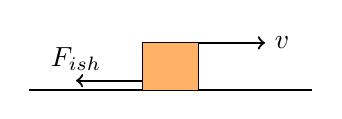
\begin{tikzpicture}[scale=0.6]

\draw[thick] (-3,0) -- (3,0);

\draw[fill=orange!60] (-0.6,0) rectangle (0.6,1);

\draw[->,thick] (0.6,1) -- (2,1);
\node[right] at (2,1) {$v$};

\draw[->,thick] (-0.6,0.2) -- (-2,0.2);
\node[above] at (-2,0.2) {$F_{ish}$};

\end{tikzpicture}

\begin{enumerate}[label=\Alph*)]
\item harakati o‘zgarmaydi
\item tekis sekinlanuvchan
\item tekis
\item tekis tezlanuvchan
\item tinch turadi
\end{enumerate}


\item Gorizontal muz ustida o‘z inersiyasi bilan sirpanib
harakat qilayotgan shayba bilan muz orasidagi
ishqalanish koeffitsiyenti 0,02 ga teng.
Shaybaning tezlanishi qanday (m/s$^2$)?

\begin{enumerate}[label=\Alph*)]
\item -0,3
\item -0,2
\item -0,03
\item -0,02
\item 0
\end{enumerate}


\item Tormozlanish yo‘li $L=\frac{v_0^2}{2\mu g}$ formula yordamida hisoblanadi. Qaysi fizik kattalik qanday o‘zgartirilsa, tormozlanish yo‘li ko‘proq kamayadi?

\begin{enumerate}[label=\Alph*)]
\item $v_0$ ni oshirib, $\mu$ kamaytirilsa
\item $v_0$ kamaytirilib, $\mu$ oshirilsa
\item $v_0$ va $\mu$ mutanosib kamaytirilsa
\item $v_0$ va $\mu$ mutanosib oshirilsa
\item $\mu$ ni o‘zgartirmay $v_0$ oshirilsa
\end{enumerate}


\item Massasi 4 kg bo‘lgan jism havoda 8,5 m/s$^2$ tezlanish bilan tushmoqda. Havoning qarshilik kuchini toping (N).

\begin{enumerate}[label=\Alph*)]
\item 34
\item 24
\item 17
\item 12
\item 6
\end{enumerate}


\item Yuqoriga tik otilgan 80 g massali jismga havoning 0,8 N qarshilik kuchi ta’sir etayotgan bo‘lsa, jismning tezlanish moduli necha m/s$^2$ ga teng?

\begin{enumerate}[label=\Alph*)]
\item 25
\item 20
\item 15
\item 10
\item 5
\end{enumerate}


\item 300 g massali jism qiya tekislik bo‘ylab yuqoriga dinamometr yordamida o‘zgarmas tezlik bilan tortilganda 3 N ni ko`rsatdi. Jism va qiya tekislik orasidagi ishqalanish koeffitsiyentini toping. $\alpha=30^\circ$,
$g=10\text{ N/kg}$.

\begin{enumerate}[label=\Alph*)]
\item 0,6
\item 0,4
\item 0,65
\item 0,58
\item 0,1
\end{enumerate}


\item Uzunligi 5 m va balandligi 3 m bo‘lgan qiya tekislikda 50 kg massali yuk turibdi. Bu yukni tutib turish uchun tekislik bo‘ylab yo‘nalgan qanday kuch qo‘yish lozim (N)? Ishqalanish koeffitsiyenti 0,2.

\begin{enumerate}[label=\Alph*)]
\item 430
\item 380
\item 250
\item 220
\item 22
\end{enumerate}


\item Ishqalanishsiz sirtdagi ikkita jismga avval $F_1$ kuch, keyin $F_1$ va $F_2$ kuchlar ta’sir qildi.
Shu ikkala holdagi ipning taranglik kuchlari nisbati $T_1/T_2$ ni aniqlang.


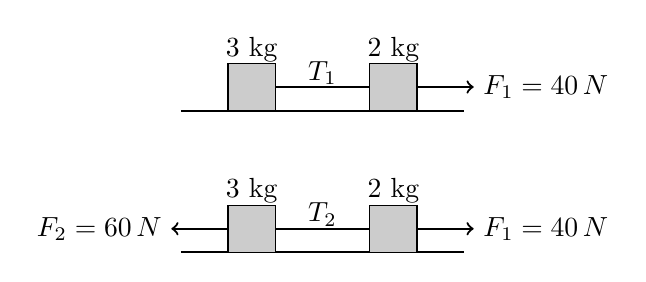
\begin{tikzpicture}[scale=0.6]

% 1-rasm
\begin{scope}[yshift=2cm]

\draw[thick] (-3,0) -- (3,0);

\draw[fill=gray!40] (-2,0) rectangle (-1,1);
\node at (-1.5,1.3) {3 kg};

\draw[fill=gray!40] (1,0) rectangle (2,1);
\node at (1.5,1.3) {2 kg};

\draw[thick] (-1,0.5) -- (1,0.5);
\node at (0,0.8) {$T_1$};

\draw[->,thick] (2,0.5) -- (3.2,0.5);
\node[right] at (3.2,0.5) {$F_1=40\,N$};

\end{scope}


% 2-rasm
\begin{scope}[yshift=-1cm]

\draw[thick] (-3,0) -- (3,0);

\draw[fill=gray!40] (-2,0) rectangle (-1,1);
\node at (-1.5,1.3) {3 kg};

\draw[fill=gray!40] (1,0) rectangle (2,1);
\node at (1.5,1.3) {2 kg};

\draw[thick] (-1,0.5) -- (1,0.5);
\node at (0,0.8) {$T_2$};

\draw[->,thick] (2,0.5) -- (3.2,0.5);
\node[right] at (3.2,0.5) {$F_1=40\,N$};

\draw[->,thick] (-2,0.5) -- (-3.2,0.5);
\node[left] at (-3.2,0.5) {$F_2=60\,N$};

\end{scope}

\end{tikzpicture}

\begin{enumerate}[label=\Alph*)]
\item 1/2
\item 2/3
\item 1
\item 3/2
\item 2
\end{enumerate}


\item Silliq gorizontal sirt ustida har birining massasi $m=10$ kg bo‘lgan va bir-biriga ip bilan bog‘langan beshta bir xil brusoklar zanjiri turibdi. Zanjir uchidagi brusokka zanjir yo‘nalishida tortuvchi $F=100$ N kuch qo‘yilgan. 1- va 2-brusokni bog‘lovchi ipning taranglik kuchi qanday (N)?

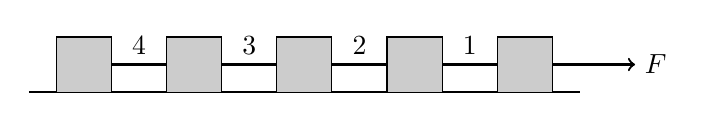
\begin{tikzpicture}[scale=0.7]

\draw[thick] (-5,0) -- (5,0);

\foreach \x/\n in {-4/4,-2/3,0/2,2/1,4/ }
\draw[fill=gray!40] (\x-0.5,0) rectangle (\x+0.5,1);

\node[above] at (-3,0.5) {4};
\node[above] at (-1,0.5) {3};
\node[above] at (1,0.5) {2};
\node[above] at (3,0.5) {1};

\foreach \x in {-3.5,-1.5,0.5,2.5}{
\draw[thick] (\x,0.5) -- (\x+1,0.5);
}

\draw[->,thick] (4.5,0.5) -- (6,0.5);
\node[right] at (6,0.5) {$F$};

\end{tikzpicture}

\begin{enumerate}[label=\Alph*)]
\item 60
\item 70
\item 80
\item 85
\item 90
\end{enumerate}


\item Rasmdagi sistemaning tezlanishini (m/s$^2$), yuqoridagi ipning taranglik kuchi $T_1$ ni (N) va $F$ kuchni (N) aniqlang. $T_2=24$ N.

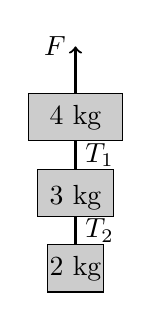
\begin{tikzpicture}[scale=0.6]

\draw[fill=gray!40] (-1,2) rectangle (1,3);
\node at (0,2.5) {4 kg};

\draw[fill=gray!40] (-0.8,0.4) rectangle (0.8,1.4);
\node at (0,0.8) {3 kg};

\draw[fill=gray!40] (-0.6,-1.2) rectangle (0.6,-0.2);
\node at (0,-0.7) {2 kg};

\draw[->,thick] (0,3) -- (0,4);
\node[left] at (0,4) {$F$};

\draw[thick] (0,2) -- (0,1.4);
\node[right] at (0,1.7) {$T_1$};

\draw[thick] (0,0.4) -- (0,-0.2);
\node[right] at (0,0.1) {$T_2$};

\end{tikzpicture}

\begin{enumerate}[label=\Alph*)]
\item 2; 6; 49
\item 2; 60; 108
\item 3; 10; 66
\item 1; 96; 29
\item 6; 96; 54
\end{enumerate}


\item Chizmadagi ipning taranglik kuchini toping.

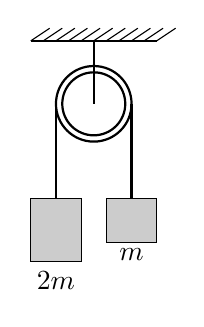
\begin{tikzpicture}[scale=0.8]

\draw[thick] (-1,3) -- (1,3);
\draw[thick] (0,2) -- (0,3);


\foreach \x in {-1,-0.8,...,1}
{
\draw (\x,3) -- (\x+0.3,3.2);
}

\draw[thick] (0,2) circle (0.6);
\draw[thick] (0,2) circle (0.5);

\draw[thick] (-0.6,2) -- (-0.6,0.5);
\draw[thick] (0.6,2) -- (0.6,0.5);

\draw[fill=gray!40] (-1,0.5) rectangle (-0.2,-0.5);
\node at (-0.6,-0.8) {$2m$};

\draw[fill=gray!40] (0.2,0.5) rectangle (1,-0.2);
\node at (0.6,-0.4) {$m$};

\end{tikzpicture}

\begin{enumerate}[label=\Alph*)]
\item $\frac{mg}{2}$
\item $\frac{2mg}{3}$
\item $mg$
\item $\frac{mg}{3}$
\item $\frac{4mg}{3}$
\end{enumerate}


\item $m_1=10$ kg, $m_2=15$ kg massali yuklar
qo‘zg‘almas vaznsiz blok orqali rasmdagidek
ipga bog‘langan.
Sistemaning tezlanishini toping (m/s$^2$).
Ishqalanishni hisobga olmang.

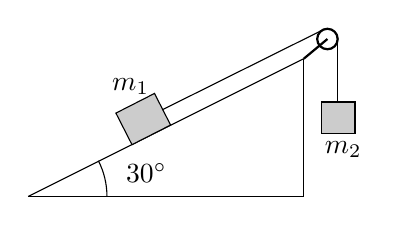
\begin{tikzpicture}[scale=1]

\draw (-3,0) -- (0.5,0);
\draw (0.5,0) -- (0.5,1.75);
\draw (-3,0) -- (0.5,1.75);

\draw (-2,0) arc (0:27:1);
\node at (-1.5,0.3) {$30^\circ$};

\draw[fill=gray!40, rotate = 27] (-1.2,1.35) rectangle (-0.65,1.8);
\node at (-1.7,1.4) {$m_1$};

\draw (-1.3,1.1) -- (0.75,2.12);

\draw[thick] (0.8,2) circle (0.13);

\draw[thick] (0.5,1.75) -- (0.8,2);
\draw (0.93,2) -- (0.93,1.2);

\draw[fill=gray!40] (0.72,0.8) rectangle (1.15,1.2);
\node at (1,0.6) {$m_2$};

\end{tikzpicture}

\begin{enumerate}[label=\Alph*)]
\item 1
\item 2
\item 4
\item 5
\item 8
\end{enumerate}


\item Ishqalanishsiz sirtdagi ikkita jism
$F$ kuch ta’sirida surib ketilmoqda.
Jismlar orasida yuzaga kelgan
ta’sir kuchini aniqlang (N).

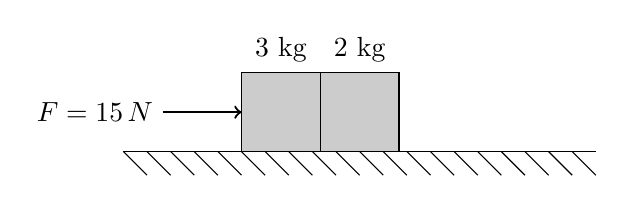
\begin{tikzpicture}[scale=1]

\draw (-3,0) -- (3,0);

\foreach \x in {-3,-2.7,...,3}
{
\draw (\x,0) -- (\x+0.3,-0.3);
}

\draw[fill=gray!40] (-1.5,0) rectangle (-0.5,1);
\node at (-1,1.3) {3 kg};

\draw[fill=gray!40] (-0.5,0) rectangle (0.5,1);
\node at (0,1.3) {2 kg};

\draw[->,thick] (-2.5,0.5) -- (-1.5,0.5);
\node[left] at (-2.5,0.5) {$F=15\,N$};

\end{tikzpicture}

\begin{enumerate}[label=\Alph*)]
\item 2
\item 6
\item 4,5
\item 3,6
\item 8
\end{enumerate}

\end{enumerate}